\documentclass[12pt]{standalone}
\usepackage[fontsize=18pt]{fontsize}
\usepackage{tikz}
\usetikzlibrary{arrows.meta}

\begin{document}
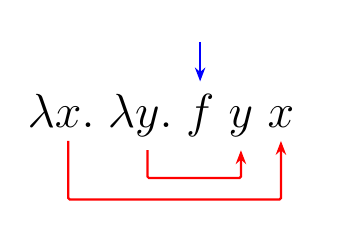
\begin{tikzpicture}[
  inner sep=0pt,
  outer sep=0pt,
  baseline=(lx.base),
]
  \path[every node/.append style={anchor=base west}]
    (0, 0)
    \foreach \name/\code in {
      tmp/\lambda,
      lx/x,
      tmp/.\;\lambda,
      ly/y,
      tmp/.\;,
      f/f,
      tmp/\ ,
      y/y,
      tmp/\ ,
      x/x,
      tmp/\ %
    } {
      node (\name) {$\code$}
      (\name.base east)
    }
  ;
  \path[
    every node/.append style={
      anchor=base,
      font=\slshape\scriptsize,
    },
  ]
    (lx.base) -- node[below=1.5\baselineskip] (bx) {} (x)
    (ly.base) -- node[below=1.1\baselineskip] (by) {} (y)
  ;
  \begin{scope}[
    >={Stealth[length=5pt]},
    thick,
    rounded corners=0.5pt,
    shorten <=.3em,
    shorten >=.3em,
  ]
    \draw[blue,->] (f.north) ++(0, 1.5em) -- (f.north);
    \def\BndArrow#1#2#3{
      \draw[red,->]
        (#2.north) ++(0, .3em) coordinate (tmp)
        (#1) |- (tmp) -| (#3)
      ;%
    }
    \BndArrow{lx}{bx}{x}
    \BndArrow{ly}{by}{y}
  \end{scope}
\end{tikzpicture}
\end{document}
